\documentclass{article}
\usepackage{paper}

\setpapertitle{Mixture of Experts using Discrete VAE}

\addauthor{Abhisek Panda}{150026}
\addauthor{Aakarsh Gajbhiye}{150067}

\begin{document}
\makeheader

\abstract{
	A lot of data in the real world exists in arbitrarily shaped clusters. Applying regression/classification models to such data can be pointless if the complexities of the hypothesis class of these models is low. Mixture of experts try to solve this problem by using a different expert/learner for each cluster, therefore creating a prediction using not one, but a mixture of learnt experts. We propose a superior gating function for these mixture of experts using Variational Autoencoders designed to perform as gating functions.
}

\begin{psection}{Introduction}

	Humans can perceive cluster patterns in data even with arbitrarily sized and shaped clusters. The same cannot be said for most machine learning models. In fact, most Mixture of Experts (ME) models are built assuming the underlying clusters of the data to be simple gaussians. This problem can, however, be alleviated by using latent variable models.

	Latent variable models essentially decode the inherent properties of the data. In the latent space, since the complexities of the data are unravelled, the clusters are simple enough to be modelled properly as gaussians. Such clustering still allows arbitrary cluster shapes in the original space.

	We use the same idea, and construct a generative model based on Variational Autoencoders(VAE) to find apt latent variables. Using this, we cluster the data, and form a simple gating function based on a Feed Forward Neural Network. The model is explained in detail in Section 3. We observe interesting results, with our model outperforming naive gating functions by a huge margin. These experiments are recorded in section 4.

\end{psection}

\begin{psection}{Background}

	\begin{psubsection}{(Generative) Latent Variable Models}
		Latent variables are variables that are not directly observed but are rather inferred from other variables that are observed \cite{wiki-latent-vars}. Suppose we have a task of creating digits (such as in MNIST), it would help to know which digit (0-9) we wish to create, what should be the width of the digit, at what angle should the digit be tilted. Such decisions can be informally called as latent variables, as these decisions, in a generative story, help us to create the digits, and in an inference story, help us understand the inherent properties of the digits.

		Such a model where we actually generate data similar to the provided training data are known as generative models. A formal description of a generative model with latent variables is described below.

		Say, we have a vector of latent variables $\vz$ in a lower-dimensional space $\cZ$, which we can easily sample according to some probability density function (pdf) $\prob{\vz}$  defined over $\cZ$. Moreover, we also have a family of deterministic functions $f(\vz; \vtheta)$, parameterized by $\vtheta$ in some space $\vTheta$, such that $f : \cZ \times \vTheta \rightarrow \cX$, where $\cX$ denotes the original data space. Our objective, therefore, is to find the correct set of parameters $\vtheta$ so that the construction of the generated data is closest to the real data. More formally, we want to find a function $f$, such that the quantity
		\begin{align*}
			\prob{\vx} = \int_\vz \prob{\vx \pipe \vz, \vtheta} \cdot \prob{\vz} \id\vz
		\end{align*}
		is maximized. For example, the probability $\prob{\vx \pipe \vz, \vtheta}$ can be formulated as $\ND{\vx \pipe f(\vz; \vtheta), \sigma^2 \vI}$ in case $\cX \in \bR $. The intuition behind this framework—called \et{maximum likelihood} is that if the model is likely to produce training set samples, then it is also likely to produce similar samples, and unlikely to produce dissimilar ones.

		Each generative model is defined by a generative story which allows us to visually interpret the interdependence of variables, more particularly dependence of observed variables on the defined latent variables.

		In most cases, the posterior of the latent variables given a data point ($\prob{\vz \pipe \vz}$) is in intractable form. In such cases, these models are trained using methods such as Monte Carlo Markov Chain(MCMC) or Variational Inference. Popular choices of generative models include variants of the vanilla Variational Autoencoder \citep{vae}. The reasons for the same are that the VAE architecture allows us to perform amortized inference (details in the next section). We take a deeper look at latent variable models in the following sections.
	\end{psubsection}

	\begin{psubsection}{Gaussian Mixture Models}
		A simple Latent Variable Model is the Gaussian Mixture Model (GMM). GMMs are useful for modeling data that come from one of several groups, with each group being modeled by a Gaussian distribution. It is used for data clustering and density estimation. The model assumes data generated for a mixture of $K$ gaussians with mixing proportion $\vpi = \brac{\pi_1 \dots \pi_K}$. Intuitively, each $\pi_k \in (0,1)$ represents the fraction of data contributed by the k\tth Gaussian.

		In this model, we define the latent variable to be the cluster assignment of each data point, \ie $z$ represents the index of the cluster the corresponding data point belongs to with a categorical/discrete prior. Therefore, the mixing proportion can now be formally defined as the weights of the categorical distribution representing the prior of the latent variable $z$. Hence, we can write
		\begin{align*}
			\prob{z = k \pipe \vpi}			&\eq \pi_k \\
			\implies \prob{z \pipe \vpi}	&\eq \prod_{k = 1}^K \para{\pi_k}^{\is{z = k}}
		\end{align*}

		Since we now have a cluster assignment, the next step is to define the probability distribution we use for sampling each data point. As pointed out earlier, this probability distribution is given by a gaussian.
		\begin{align*}
			\prob{\vx \pipe z = k} \eq \ND{\vx \pipe \vmu_k, \vSigma_k^{-1}}
		\end{align*}

		Since doing straight-forward MLE is not possible for this model (due to the presence of latent-variables), we estimate the parameters $\set{\vmu_k, \Sigma_k}_{k = 1}^K$ using Expectation Maximization(EM) Algorithm, which is a popular strategy for simple latent-variable models.

		The problem with GMM is the assumed Gaussian structures for each cluster. As pointed out earlier, this limits the power of GMM therefore not allowing arbitrary clustered data to be modeled using such models. We therefore need to explore other latent variable models with higher reprentational/expressive power. One such model is the Variational Deep Embeddings (VaDE) Model \citep{vade}, based on the Variational Autoencoder architecture. We discuss this model in the next section.
	\end{psubsection}

	\begin{psubsection}{Variational Autoencoders}
		Variational Autoencoders were initially proposed by \cite{vae}. The key idea behind VAEs is that any distribution in $D$ dimensions can be generated by taking a set of $D$ variables that are normally distributed and mapping them through a sufficiently complicated function \citep{vae-tut}. Hence, provided powerful function approximators, we can simply learn a function which maps independent, normally distributed variables to the latent variables needed for our model, and these latent variables are then used to model the observations $\vX$, or rather the data distribution $\cD$ not known to us, from which the observations are assumed to be sampled.

		The task, therfore, is to find a strong non-linear mapping to approximate the latent variables needed to model the data distribution $\cD$. This mapping, in VAEs, is modelled using a neural network, and the mapping from these latent variables to the observations is through a distribution (generally exponential family) depending on the observed space $\cX$. For example, if $\cX \in \bR$, then the estimated probability distribution for $\vx \sim \cD$ can be given as
		\begin{align*}
			\prob{\vx \pipe \vz} \eq \ND{\vx \pipe f(\vz; \vtheta), \sigma^2 \vI}
		\end{align*}
		for some non-linear mapping $f: \bR \ra \bR$ (in this case) modelled using a neural network.

		The objective now is to compute the posterior over $\vz$ given the observation $\vx$. This would allow us to model the predictive posterior using samples of $\vz$ from this posterior. Since the posterior $\prob{\vz \pipe \cD}$ is intractable, we approximate it using a proposal distribution $\cQ\para{\vz \pipe \vx, \vphi}$. We use the standard Black Box Variational Inference strategy to estimate the posterior, by maximizing the ELBO bound using descent methods, which is given as
		\begin{align*}
			\cL(\vx; \cQ) &\eq \log{\prob{\vx}} - \text{KL}\brac{\cQ\para{\vz; \vphi}\ ||\ \prob{\vz \pipe \vx}} \\
			&\eq \E[\vz \sim \cQ\para{\vz \spipe \vx, \vpi}]{\log{\frac{\prob{\vx, \vz}}{\cQ\para{\vz \pipe \vx, \vphi}}}}
		\end{align*}
		Typically, the prior over the latent variables $\vz$ is assumed to be a multivariate normal distribution with mean $\vzero$ and variance matrix $\vI$.

		This structure is similar to that of a standard autoencoder, where the network which maps the inputs to the parameters of the proposal is the encoder and the network mapping the sampled $\vz$'s to the parameters of the conditional likelihood distribution is the decoder.

		One major problem with Variational Inference is that it models the parameters of each latent variable independently, and therefore we need an iterative procedure to model the proposal with respect to each variable. That is, if we want to add a new data point, we need to remodel the proposal in order to compute the pdf of the new latent variable. VAE tackles this problem by assuming that the latent variable is dependent on the input, and the mapping from the input to the parameters of the proposal distribution is modeled using a neural network. This, essentially, is the idea of amortized inference.

		Since looking at the ELBO, one can say we wish to minimize the KL Divergence between the proposal and the prior for $\vz$ which is a standard Normal distribution, we can assume the proposal to be of the form \ $\ND{\vz \pipe \vmu(\vx; \vphi), {\vsigma}^2(\vx; \phi) \vI}$. The negative ELBO is then considered as our loss, and the parameters (or weights) of the Neural Networks are inferred.

		However, since we are assuming the variables $\vz$ to be sampled from the proposal, we cannot apply back propogation across the decoder and the encoder networks. This is handled using the reparameterization trick, where we write $\vz = \vepsilon \cdot {\vsigma}^2(\vx; \vphi) + \vmu(\vx; \vphi)$. This allows us to input the reparametrized latent variables $\vepsilon$, and therefore facilitate backpropogation through the stochastic nodes. The working of a standard VAE is visuallized in figure \ref{fig:VAE} \footnote{Image taken from \cite{vae-tut}}.

		\begin{figure}
			\centering
			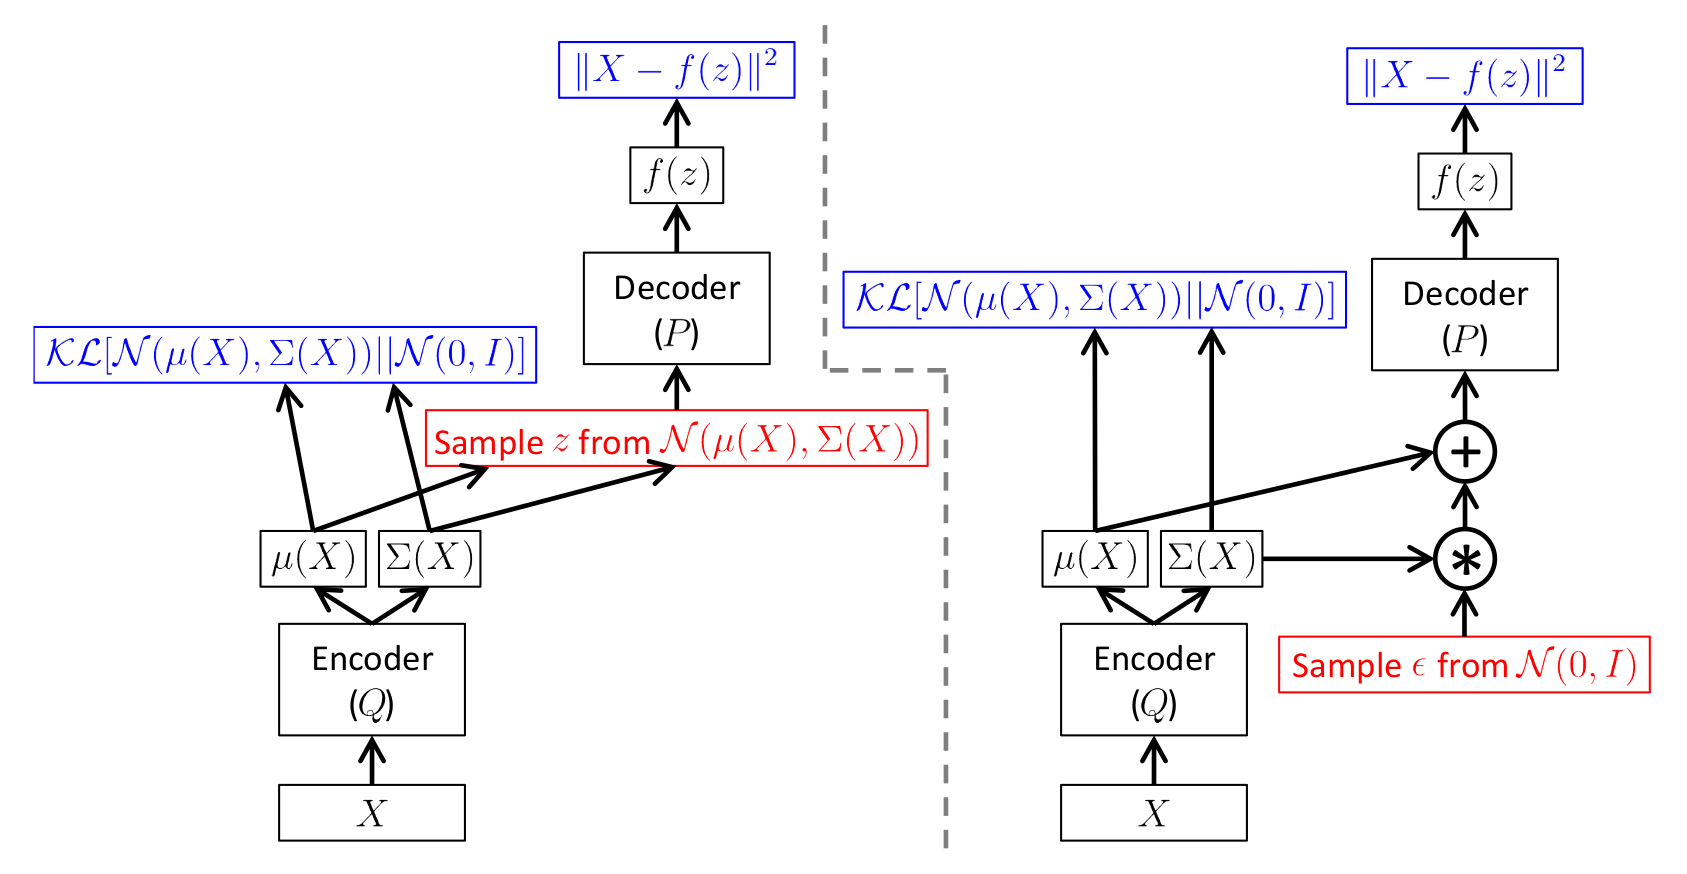
\includegraphics[width=0.9\textwidth]{includes/vae.png}
			\caption{Without (left) and with (right) the reparametrization trick}
			\label{fig:VAE}
		\end{figure}

	\end{psubsection}

\end{psection}

\begin{psection}{Variational Deep Embeddings}

	\begin{algo}[0.9\textwidth]{Generative Story}

		The generative story for a mixture madel based on latent variables can be written as
		\begin{align*}
			c				&\qsim \text{Cat}\para{\vpi} \\
			\vz \pipe c = k	&\qsim \ND{\vz \pipe \vmu_k, \Sigma_k} \\
			\vx \pipe \vz	&\qsim p\para{\vx \pipe \func{f}{\vz; \vphi}, \func{f}{\vz; \vphi}}
		\end{align*}

		In our case, we model the function $f$ using a neural network. The probability distribution $p$ can be any distribution which is apt for the data space. For example, if the data space is real, \ie $\cx = \bR$, then the probability distribution can be a Gaussian, with the function $f$ feeding the mean and the variance of the gaussian.

	\end{algo}

	Variational Deep Embedding (VaDE) was proposed by \cite{vade}. It is a simplistic model than the previous models discussed, and greatly simplifies the generic generative story by assuming a uniform prior on the cluster means, variances, and misture proportions. Also, it assumes a uniform prior on the model parameters $\vtheta$.

	\begin{figure}[h]
		\centering
		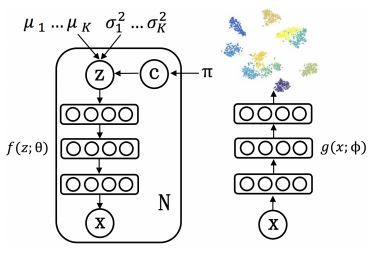
\includegraphics[height=150px]{includes/vade.jpg}
		\caption{Plate notation for VaDE (left) and an encoder network $g(\vx; \phi) (right)$}
		\label{fig:my_label}
	\end{figure}

	Depending on whether the observations $\vx$ is binary or real-valued we compute $\mu_x = f(\vz, \vtheta)$ and choose a sample $\vx \sim Ber(\mu_x)$ or compute $[\mu_x;\log\sigma^2_x] = f(\vz,\vtheta)$ and choose a sample $\vx \sim \mathcal{N}(\mu_x,\sigma^2_x\vI)$. From the generative story, the joint probability can be written as
	\begin{align*}
		\prob{\vx, \vz, c} \eq \prob{\vx \pipe \vz, \vtheta} \prob{\vz \pipe c} \prob{c}
	\end{align*}

	An instance of VaDE is tuned to maximize the likelihood of the given data points. Given the generative process described above we have
	\begin{align*}
		\logp{\prob{\vx}} &\eq \log{\int_\vz \sum_c \prob{\vx, \vz, c} \id \vz} \\
		&\qge \E[\cQ\para{\vz, c \spipe \vx}]{\logp{\frac{\prob{\vx, \vz, c}}{\cQ\para{\vz, c \pipe \vx}}}} \eq \cL_{\text{ELBO}}
	\end{align*}
	where $\cQ\para{\vz, c \pipe \vx}$ is the proposal distribution.

	Mean field is assumed on the proposal distribution, giving:
	\begin{align*}
		\cQ\para{\vz, c \pipe \vx} &\eq \cQ\para{\vz \pipe \vx} \cQ\para{c \pipe \vx}
	\end{align*}

	Similar to VAE, the distribution $\cQ\para{\vz \pipe \vx}$ is modelled using a neural network $g$ as follows
	\begin{align*}
		\tilde{\vmu}, \logp{\tilde{\vsigma}^2} &\eq g(\vx, \vphi) \\
		\cQ\para{\vz \pipe \vx} &\eq \ND{\vz \pipe \tilde{\vmu}, \tilde{\vsigma}^2 \vI}.
	\end{align*}

	Further, a decoder model is added giving the following:
	\begin{align*}
		\prob{\vx \pipe \vz} &\eq \prob{\vx \pipe f(\vz, \vtheta)}
	\end{align*}

	The authors use an interesting approach to ``approximating'' the proposal distribution $\cQ\para{c \pipe \vx}$, which although looks absurd, in practice works surprisingly well. First, one can realize, the ELBO can be re-written in the following manner,
	\begin{align*}
		\cL_{\text{ELBO}} &\eq 	\E[\cQ\para{\vz, c \spipe \vx}]{\logp{\frac{\prob{\vx, \vz, c}}{\cQ\para{\vz, c \pipe \vx}}}} \\
		&\eq					\int_{\vz} \sum_{c} \cQ\para{c \pipe \vx} \cQ\para{\vz \pipe \vx} \set{\logp{\frac{\prob{\vx \pipe \vz} \prob{\vz}}{\cQ\para{\vz \pipe \vx}}} + \logp{\frac{\prob{c \pipe \vz}}{\cQ\para{c \pipe \vx}}}} \\
		&\eq \int_{\vz} \cQ\para{\vz \pipe \vx} \logp{\frac{\prob{\vx \pipe \vz} \prob{\vz}}{\cQ\para{\vz \pipe \vx}}} \id \vz - \int_{\vz} \cQ\para{\vz \pipe \vx} \kld{\cQ\para{c \pipe \vx}}{\prob{c \pipe \vz}} \id \vz
	\end{align*}

	In order to maximize the above ELBO, it seems we need to minimize the average KL Divergence over the latent variables, when sampled using the posterior. \et{Jiang et al.} approximated this simply using only one sample of $\vz$ and therefore, we can write
	\begin{align*}
		\cQ\para{c \pipe \vx} \eq \prob{c \pipe \vz = \hat{\vz}} \eq \frac{\prob{c} \prob{\vz = \hat{\vz} \pipe c}}{\sum_{c' = 1}^{K} \prob{c'} \prob{\vz = \hat{\vz} \pipe c'}}
	\end{align*}
	where $\hat{\vz}$ is a sample from the posterior proposal $\cQ\para{\vz \pipe \vx}$.

	Given the simplicity of the model, we performed some experiments on it. We implemented the complete model on Tensorflow from scratch, and performed experiments on a couple of datasets. This is discussed in detail in the following section.
\end{psection}

\begin{psection}{Mixture of Experts (ME)}
	Just like GMM, a mixture of experts model splits the data into soft clusters, and for each cluster, we have an expert which predicts the target labels for each mixture. Therefore, we need to define a \et{gating function}, which defines the mixing proportions for each data point. Suppose we denote the mixture assignment using a latent variable $c$, then we have a probability density/mass function $\prob{\vy \pipe \vx, c}$. Mostly this probability is defined using a pdf function belonging to the class of exponential distributions. For example, if the space of the target label $\cY = \set{0, 1}$, then we can define $\prob{\vy \pipe \vx, c}$ to be a Bernoulli distribution.

	We still need to define a mixing proportion. Since our ultimate goal is to model $\prob{\vy \pipe \vx}$, we write
	\begin{align*}
		\prob{\vy \pipe \vx} &\eq \sum_{k = 1}^K \prob{\vy, c = k \pipe \vx} \\
		&\eq \sum_{k = 1}^K \prob{c \pipe \vx} \cdot \prob{\vy \pipe c = k, \vx}
	\end{align*}

	Looking at the above equation, we can say setting $\prob{c \pipe \vx}$ to be the mixing proportion as a natural choice. The most common choice for modelling this probability mass function is using a softmax distribution as follows -
	\begin{align*}
		\prob{c = k \pipe \vx} \eq \frac{\texp{b_k + \dotp{\vw_k}{\vx}}}{\sum_{k' = 1}^K \texp{b_{k'} + \dotp{\vw_{k'}}{\vx}}}
	\end{align*}
	where K is the number of experts.

	We usually represent $\prob{c = k \pipe \vx}$ using the function $g_k(\vx, \vTheta_g)$. To sum up ME models, $g_k(\vx, \vTheta_g)$ is essentially the gate's rating for the k\tth expert given $\vx$ and $\prob{\vy \pipe \vx, c, \vTheta_e}$ is the probability of the k\tth expert generating $\vy$ given $\vx$. For brevity, we denote this as $p_i(\vy)$.

	In general, the ME training algorithm maximizes the log-likelihood $\prob{\vy \pipe \vx}$ to learn the parameters of the expert and the gate. During the training ME, the gate and the experts gets decoupled, therefore the model attains a modular structure. This property is exploited in order to extend ME models to hierarchical mixture of experts (HME). A standard ME model is graphically represented in figure \ref{fig:me} \footnote{Image taken from \cite{me-image}}.

	\begin{figure}[htpb]
		\centering
		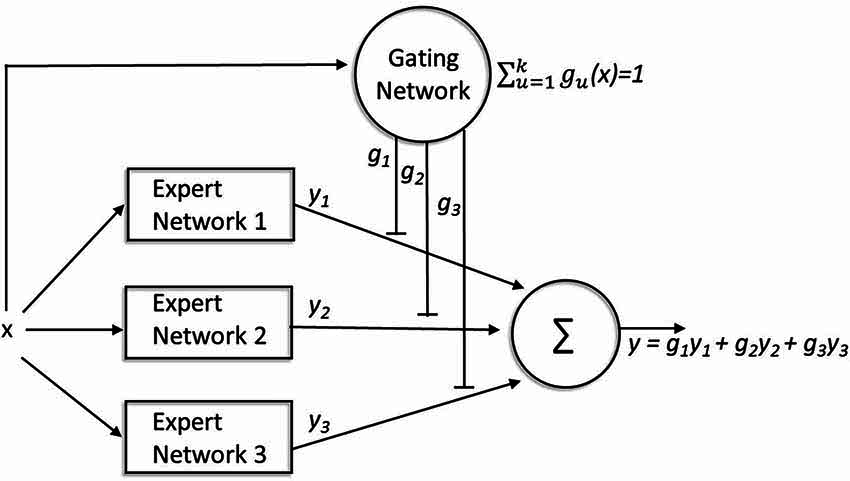
\includegraphics[width=0.7\textwidth]{includes/me.png}
		\caption{Graphical representaion of a standard Mixture of Experts model}
		\label{fig:me}
	\end{figure}

	\begin{psubsection}{ME Regression Model}

		Let $\vTheta_e = \set{\sW_k, \Gamma_k}_{k = 1}^{K}$ denote the parameters of the experts. As mentioned earlier, in the original ME regression model, the experts follow the gaussian model -
		\begin{align*}
			\prob{\vy \pipe \vx, c = k} \eq \ND{\vy \pipe \hat{\vy}(\vx, \sW_k), \Gamma_k}
		\end{align*}
		where $\vy \in \bR^\sM$. The term $\hat{\vy}(\vx, \sW)$ is defined as $\hat{\vy}(\vx, \sW) = \sW \vx$. We can also add a bias term to $\sW \vx$.

		At test time, in order to make a prediction, the expectation of $\vy$ with respect to the pdf $\prob{\vy \pipe \vx,\vTheta}$ is used as the output of the architecture. This is, therefore, given by
		\begin{align*}
			\hat{\vy} = \sum_{k = 1}^K g_k(\vx, \vTheta_g) \cdot \hat{\vy}(\vx, \sW)
		\end{align*}
	\end{psubsection}

	\begin{psubsection}{ME Classification Model}
		In this case, the probability of $\vy$ is given by a categorical/discrete distribution. In the one hot representation, the desired output $\vy$ is of length L and $y_l$ = 1 if $\vx$ belongs to class $l$ and 0 otherwise. Also, expert $k$ has parameters $\set{\vw_{imk}}_{k = 1}^K$, corresponding to the parameters of each class. The probability given by each expert is therefore written as
		\begin{align*}
			\prob{\vy \pipe \vx, c = k} &\eq \prod_{l = 1}^L \hat{\vy_l}(\vx, b_k, \vw_k)^{\is{y_l = 1}} \\
			\hat{\vy_l} &\eq \frac{\texp{\dotp{\vw_{ik}}{\vx}}}{\sum_{l' = 1}^L \texp{\dotp{\vw_k}{\vx}}}
		\end{align*}

		The prediction is done in the same way as was shown for the ME Regression Model.

	\end{psubsection}

	Although the paradigm of Mixture of Experts is very generic, not many methods exist for the same. The fundamental problems are the difficulties of inference, along with non-compatibility with automatic differentiation libraries for the existing inference methods. We try to remedy this problem by proposing a novel Mixture of Experts model based on Variational Autoencoders. In the next section, we show a way to extend the VaDE model for use as a gating function for ME models, and point out some difficulties in doing the same. Following that, we propose a novel gating function based on Discrete Latent Variables in Variational Autoencoders, and later show that it outperforms other naive gating functions.
\end{psection}

\begin{psection}{VaDE with Mixture of Experts}
	The VaDE model originally described in \cite{vade} is used to learn cluster assignments and also works as a generative model. For using VaDE in classification/regression tasks, the original theory can be extended in a straight-forward manner by maximizing an appropriate loss function. This loss function needs to include the predicted label ($\vy$) along with reconstruction of $\vx$. Although general learning models would maximise the log-likelihood \ie $\prob{\vy \pipe \vx}$, we are aiming to build a generative model and therefore our maximization objective will be $\prob{\vx, \vy}$.
	\begin{align*}
		\logp{\prob{\vx, \vy}} &\eq \log{\int_\vz \sum_c\prob{\vx, \vy, \vz, c}} \\
		&\qge \E[\cQ\para{\vz, c \spipe \vx, \vy}]{\logp{\frac{\prob{\vx, \vy, \vz, c}}{\cQ\para{\vz, c \pipe \vx, \vy}}}}\\
		&\eq \E[\cQ\para{\vz, c \spipe \vx, \vy}]{\logp{\prob{\vy \pipe \vx, \vz, c}}} + \E[\cQ\para{\vz, c \spipe \vx, \vy}]{\logp{\frac{\prob{\vx, \vz, c}}{\cQ\para{\vz, c \pipe \vx, \vy}}}} \\
		&\eq \cL_{\text{ELBO}}
	\end{align*}
	Note that the second part of this formulation closely resembles the original $\cL_{\text{ELBO}}$, except for an additional $\vy$ term in the proposal distribution. The proposal distribution $\cQ$ can be modelled as follows:
	\begin{align*}
		\cQ\para{\vz, c \pipe \vx, \vy} &= \cQ\para{c \pipe \vx, \vy}\cQ\para{\vz \pipe \vx, \vy, c}
	\end{align*}
	Again, assuming Mean Field approximation, we can write $\cQ\para{\vz \pipe \vx, \vy, c} = \cQ\para{\vz \pipe \vx, \vy}$. Further, the latent representation $\vz$ can be assumed to be independent of $\vy$ conditioned on $\vx$. So, we can further simplify $ \cQ\para{\vz \pipe \vx, \vy} = \cQ\para{\vz \pipe \vx}$

	The estimate for $\cQ\para{c \pipe \vx, \vy}$ remains exactly the same as that of $\cQ\para{c \pipe \vx}$ in the original VaDE model, and is approximated as:
	\begin{align*}
		\cQ\para{c \pipe \vx, \vy} \eq \prob{c \pipe \vz = \hat{\vz}} \eq \frac{\prob{c} \prob{\vz = \hat{\vz} \pipe c}}{\sum_{c' = 1}^{K} \prob{c'} \prob{\vz = \hat{\vz} \pipe c'}}
	\end{align*}
% NOTE: show derivation if needed

	Therefore, the second part remains exactly same as that of the original VaDE model. The first part of $\cL_{\text{ELBO}}$ is the familiar supervised learning term. Since $\vy$ can be assumed to depend only on $\vx$ and $c$, we have:
	$$ \prob{\vy \pipe \vx, \vz, c} = \prob{\vy \pipe \vx, c} $$
	Depending on the task at hand, $\prob{\vy \pipe \vx, c}$ can be modelled in various ways. For a regression task, we can use a linear model $\left\{ \vW_c, \vb_c \right\}_{c=1}^{K}$, so that maximizing $\prob{\vy \pipe \vx, c}$ is equivalent to minimizing $ \left(\hat{\vy} - \para{\vW_c\vx + \vb_c}\right)^2$

	\begin{psubsection}{Test Time Approximations}
		During test time, we have to estimate $\prob{\vy \pipe \vx}$. We can wirte this as follows:
		\begin{align*}
			\prob{\vy \pipe \vx} &\eq \sum_c \prob{c\pipe\vx}\prob{\vy \pipe \vx, c} \\
			&\eq \sum_c \para{\int_{\vz} \prob{c\pipe\vx, \vz}\prob{\vz \pipe \vx}}\prob{\vy \pipe \vx, c}\\
			&\eq \sum_c \para{\E[\prob{\vz \pipe \vx}]{\prob{c\pipe\vz}}}\prob{\vy \pipe \vx, c}
		\end{align*}
		We again assume that $c$ is independent of $\vx$ conditioned on $\vz$. Further, we can use monte carlo estimates to compute the expectation, and $\prob{c\pipe\vz}$ is estimated using the same approximation as that used during inference.
	\end{psubsection}

	\begin{psubsection}{Shortcomings of VaDE model}
		A major shortcoming of the VaDE model is using a single sample to approximate $\cQ\para{c \pipe \vx, \vy}$. The requirement for zeroing out the KL divergence is that $\cQ\para{c \pipe \vx, \vy}$ is exactly equal to $\prob{c \pipe \vz}$ at all points, which is not true in general. However, using a single $\hat{\vz}$ introduces deviations from actual value which leads to slow inference.

		Also, during test time, we need to approximate $\mathbb{E}_{\mathbb{P}[\vz \pipe \vx]}{\prob{c\pipe\vz}}$ which uses the same approximation along with monte carlo estimates which are known to have high variance. Hence, this may lead to inaccuracies during test time.
	\end{psubsection}
\end{psection}

\begin{psection}{Discrete Mixture Variational Autoencoders}

	As pointed out in the previous section, a gating function based on VaDE will suffer from two prime problems, slow inference and slow and inaccurate predictions. We try to design a gating function keeping these two problems in mind.

	We follow the same generative story as outlined in algorithm \hyperlink{algo:1}{1}, and use the same mean-field assumption as VaDE, \ie $\cQ\para{\vz, c \pipe \vx} = \cQ\para{\vz \pipe \vx} q(c \pipe \vx)$. Therefore, we can write the ELBO in the same way oulined in VaDE.

	In order to tackle the problems in VaDE, we propose to add a separate encoder network for inferring the latent variable $c$, \ie the cluster assignment. The sole problem in the formulation is the discontinuous nature of the latent variable $c$. Since the variable is a categorical one, it is not possible to find a deterministic reparametrization formulation, we cannot use backpropogation over this stochastic node. However, there exist methods which facilitate black box variational inference with binary/categorical stochastic nodes.

	The most popular strategy to facilitate BBVI, and therefore backpropogation over discrete nodes is Gumbel-Softmax. Briefly, the gumbel-softmax trick relaxes the discrete variables to continuous ones, and allow backpropogation through an appropriate reparametrization function. The details of this trick are mentioned in the following section.

	\begin{psubsection}{Gumbel Softmax Trick}

		As mentioned, we need to find a smooth relaxation for discrete latent variables, along with an apt reparametrization variable to allow backpropogation, and therefore inference using black box variational inference for a model.

		Firstly, we need to look at how we can sample from a categorical (consider single dimension) variable. The typical way of doing so would be to sample a uniform random variable (from 0 to 1), U and return the categorical variable as follows
		\begin{align*}
			\sC \eq \argmin{k \in \brac{K}} \sU - \sum_{k' = 1}^k \pi_{k'}
		\end{align*}

		\note{The parameters $\set{\pi_k}_{k = 1}^K$ denote the probabilities of each class for the categorical distribution, and therefore $\sum_{k = 1}^K \pi_k = 1$. Below, we alternately use weights $\set{\alpha_k}_{k = 1}^K$ instead of probabilities, and therefore, we will have $\pi_k = \frac{\alpha_k}{\sum_{k' = 1}^{K} \alpha_{k'}}$}

		An alternate way, however, to sample from the categorical distribution is by using the Gumbel-Max trick (upon which the Gumbel-Softmax is based). The Gumbel-Max trick says that in order to sample from a categorical distribution with weights $\set{\alpha_k}_{k = 1}^K$, we sample $K$ uniform random variables $\set{\sU_k}_{k = 1}^{K}$ and reparametrize as follows
		\begin{align*}
			\sC \eq \argmax{k \in \brac{K}} \log{\alpha_k} - \log{- \log{\sU_k}}
		\end{align*}

		The variable $-\log{-\log{U}}$ is known to be from the Gumbel disitribution. This alternate sampling strategy allows us to write the relaxed version of the random variable C (denoted by $\vZ = \brac{\sZ_1 \dots \sZ_K}$). which is then given as
		\begin{align*}
			\sZ_k \eq \frac{\texp{\para{\log{\alpha_k} + \sG_k} / \tau}}{\sum_{k' = 1}^K \texp{\para{\log{\alpha_{k'}} + \sG_{k'}} / \tau}}
		\end{align*}
		where $\sG_k$ is a sample from the gumbel distribution, and $\tau$ is a parameter, known as the temperature. It is obvious to see that as $\tau \ra 0$, the smooth relaxation $Z_k \ra \is{C = k}$.

		Following other details from the Concrete paper, we are able to train VAEs with (relaxed) discrete latent variables. This, now. allows us to model the posterior for the latent variable $c$ using an encoder network.

	\end{psubsection}

	As we have an estimate of the posterior of all the latent variables, we do not need an approximation to compute $\cQ\para{c \pipe \vx}$ as was the case in VaDE. The remaining model remains the same, with K means and variances as the prior parameters, and the same KL computation as in VaDE. One difference, however, we have from VaDE is that we have a uniform prior on the category probabilities, \ie, in the prior for $c$, we assume each cluster to have equal probability. This can, however, be easily removed as it does not change the computations at any point. We call this model Discrete Mixture Variational Autoencoder (DMVAE).

	Modelling the posterior of the latent variable C allows faster inference possible. We document the difference in inference time and results between DMVAE and VaDE in section 8. Our hypothesis is that this occurs due to the added noise in approximating $\cQ\para{c \pipe \vx}$ using a single sample. If we take a look at the expanded ELBO term in the VaDE paper (for normal distribution over $\vx \pipe \vz$), it shows a similar problem Black Box Variational Inference faces without reparametrization. Due to the shortage of time, we could not emperically confirm this hypothesis but the faster inference for DMVAE endorses this hypothesis.

	This formulation of DMVAE easily extends to Mixture of Experts models with the DMVAE model as a variational gating function. We look at the details of the same in the next section.

\end{psection}

\begin{psection}{Mixture of Experts with DMVAE}

	Since we do not alter the general formulation of the ME models, we can still write the basic equations. That is, for some latent variable C denoting the cluster/mixture assignment, we have
	\begin{align*}
		\prob{\vy \pipe \vx} \eq \sum_{k = 1}^{K} \prob{c = k \pipe \vx} \prob{\vy \pipe \vx, c = k}
	\end{align*}

	As discussed in earlier sections, we can model $\vy \pipe \vx, c$ using an appropriate distribution (commonly exponential family). The posterior probabily for cluster assingment. in case of VaDE, caused problems during test time, as discussed. In case of DMVAE, we avoid this problem by approximating the posterior using a neural network (encoder network). This, therefore, saves time during prediction by avoiding sampling of latent variable $Z$.

	Morevover, we still use the mean field assumption, same as VaDE. However, for the case of ME with DMVAE, we estimate the posterior $\prob{\vz, c \pipe \vx, \vy}$ using $\cQ\para{\vz, c \pipe \vx, \vy}$ having the following assumptions
	\begin{align*}
		\cQ\para{\vz, c \pipe \vx, \vy} &\eq \cQ\para{\vz, c \pipe \vx} \\
		&\eq \cQ\para{\vz \pipe \vx} \cQ\para{c \pipe \vx}
	\end{align*}

	We can now write the loss function. Similar to VaDE based ME, we need to maximize the probability $\prob{\vx, \vy}$. However, since we now can compute the exact (estimate of) posterior $\cQ\para{c \pipe \vx}$, we can alter the lower bound to be tighter than the ELBO term used for ME with VaDE. This also has an additional benifit highlighted later in this section. This altered lower bound can be written as
	\begin{align*}
		\logp{\prob{\vy, \vx}} &\eq \logp{\prob{\vy \pipe \vx}} + \logp{\prob{\vx}} \\
		&\qge	\logp{\prob{\vy \pipe \vx}} + \E[\vz, c \spipe \vx]{\log{\frac{\prob{\vz, c, \vx}}{\cQ\para{\vz, c \pipe \vx}}}} \\
		&\eq	\logp{\prob{\vy \pipe \vx}} + \E[\vz, c \spipe \vx]{\logp{\prob{\vx \pipe \vz, c}} + \log{\frac{\prob{\vz \pipe c}}{\cQ\para{\vz \pipe \vx}}} + \log{\frac{\prob{c}}{\cQ\para{c \pipe \vx}}}} \\
		\cL(\vx, \vy)	&\eq	\logp{\prob{\vy \pipe \vx}} + \E[\vz \spipe \vx]{\logp{\prob{\vx \pipe \vz}}} - \E[c \spipe \vx]{\kld{\cQ\para{\vz \pipe \vx}}{\prob{\vz \pipe c}}} \\&\hspace{1.1cm}- \kld{\cQ\para{c \pipe \vx}}{\prob{c}}
	\end{align*}

	Each term can be intuitively understood, with the first term maximizing the likelihood, the second term maximizing the reconstruction power of the VAE, the third term ensuring low divergence between the prior cluster mean and the posterior encoded mean, and the last term ensuring low divergence between the mixing proportions in the prior and the posterior for the latent variable C.

	The third term has the prior conditioned on C for each KL Divergence term. This conditioning is not deterministic on the mixing proportions (encoder network for C), and therefore we replace C (for this term) with its smooth relaxation using the Gumbel-Softmax Trick, say $\zeta$. Since $\zeta$ is continuous and we cannot comput the expectation term analytically, we need to use Monte Carlo tricks, same as what is done for Z in a standard VAE (and will be done for the second term here as well). We can, therefore, write the relaxed object $\widetilde{\cL}$ as follows
	\begin{align*}
		\widetilde{\cL}(\vx, \vy)		&\eq	\logp{\prob{\vy \pipe \vx}} + \E[\vz \spipe \vx]{\logp{\prob{\vx \pipe \vz}}} - \E[\vz, \vzeta \spipe \vx]{\kld{\cQ\para{\vz \pipe \vx}}{\prob{\vz \pipe \vzeta}}} \\&\hspace{1.1cm}- \kld{\cQ\para{c \pipe \vx}}{\prob{c}}
	\end{align*}

	Although $\widetilde{\cL}$ isn't necessarily a lower bound for the objective $\logp{\prob{\vx, \vy}}$, however, empirically it seems to work (section 8).

	\note{We must ensure the relaxed prior probability $\prob{\vz \pipe \vzeta}$ limits to $\prob{\vz \pipe c}$ as $\tau \ra 0$}

	\bt{Advantages of Using DMVAE as a gating function}
	\begin{enumerate}
			\ditem[Automatic Differentiation] Use of Black Box Variational Inference with the reparametrization and gumbel trick allows us to use automaic differentiation libraries (such as Tensorflow) to compute the gradients and therefore infer the parameters of the model using gradient based techniques. This is not possible with models using the EM algorithm, as the updates need to be manually coded.
			\ditem[Handling of Arbitrary Shaped Clusters] As pointed out earlier, clustering in latent space with non-linear transformations (decoder) allows us to even cluster data split in arbitrary shaped clusters. DMVAE, therefore accurately handles clustering of data at least as good as some other non-trivial models (such as VaDE). This also helps in learning mixture of experts models where the data is complicated or high-dimensional.
			\ditem[Fast Inference] Since VAEs, and henceforth DMVAE, use amortized inference and reparametrization, the inference is usually fast. Coupled with automatic differentiation, this affors a ``nice'' model for ME and/or clustering tasks.
	\end{enumerate}

\end{psection}


\begin{psection}{Experiments}
	We conducted a variety of experiments to test the robustness of our algorithm. The datasets we use for these tasks are MNIST \cite{<++>} and spiral dataset. Firstly, we show some experiments on VaDE and DMVAE showing reconstruction and generation powers of the models. Later, we show the effectiveness of DMVAE over naive gating functions for ME.

	\begin{psubsection}{VAE Training}
		The VaDE and DMVAE models in addition to learning cluster assignments also allow us to generate new data points. This section details our findings of how well these models learnt to reconstruct the original image along with their power to produce new novel images.
		\begin{pssubsection}{MNIST Dataset}
			The MNIST dataset contains 60,000 training images and 10,000 testing images, each image being greyscaled and of size $28 \times 28$. The images represent digits from 0 to 9, and are labelled accordingly.

			Figures \ref{fig:dmvae_mnist_regen} and \ref{fig:vade_mnist_regen} show the reconstruction power of DMVAE and VaDE models, respectively, trained using MNIST dataset. It can be clearly seen that both models have learnt to reproduce images well.
			\begin{figure}[H]
				\centering
				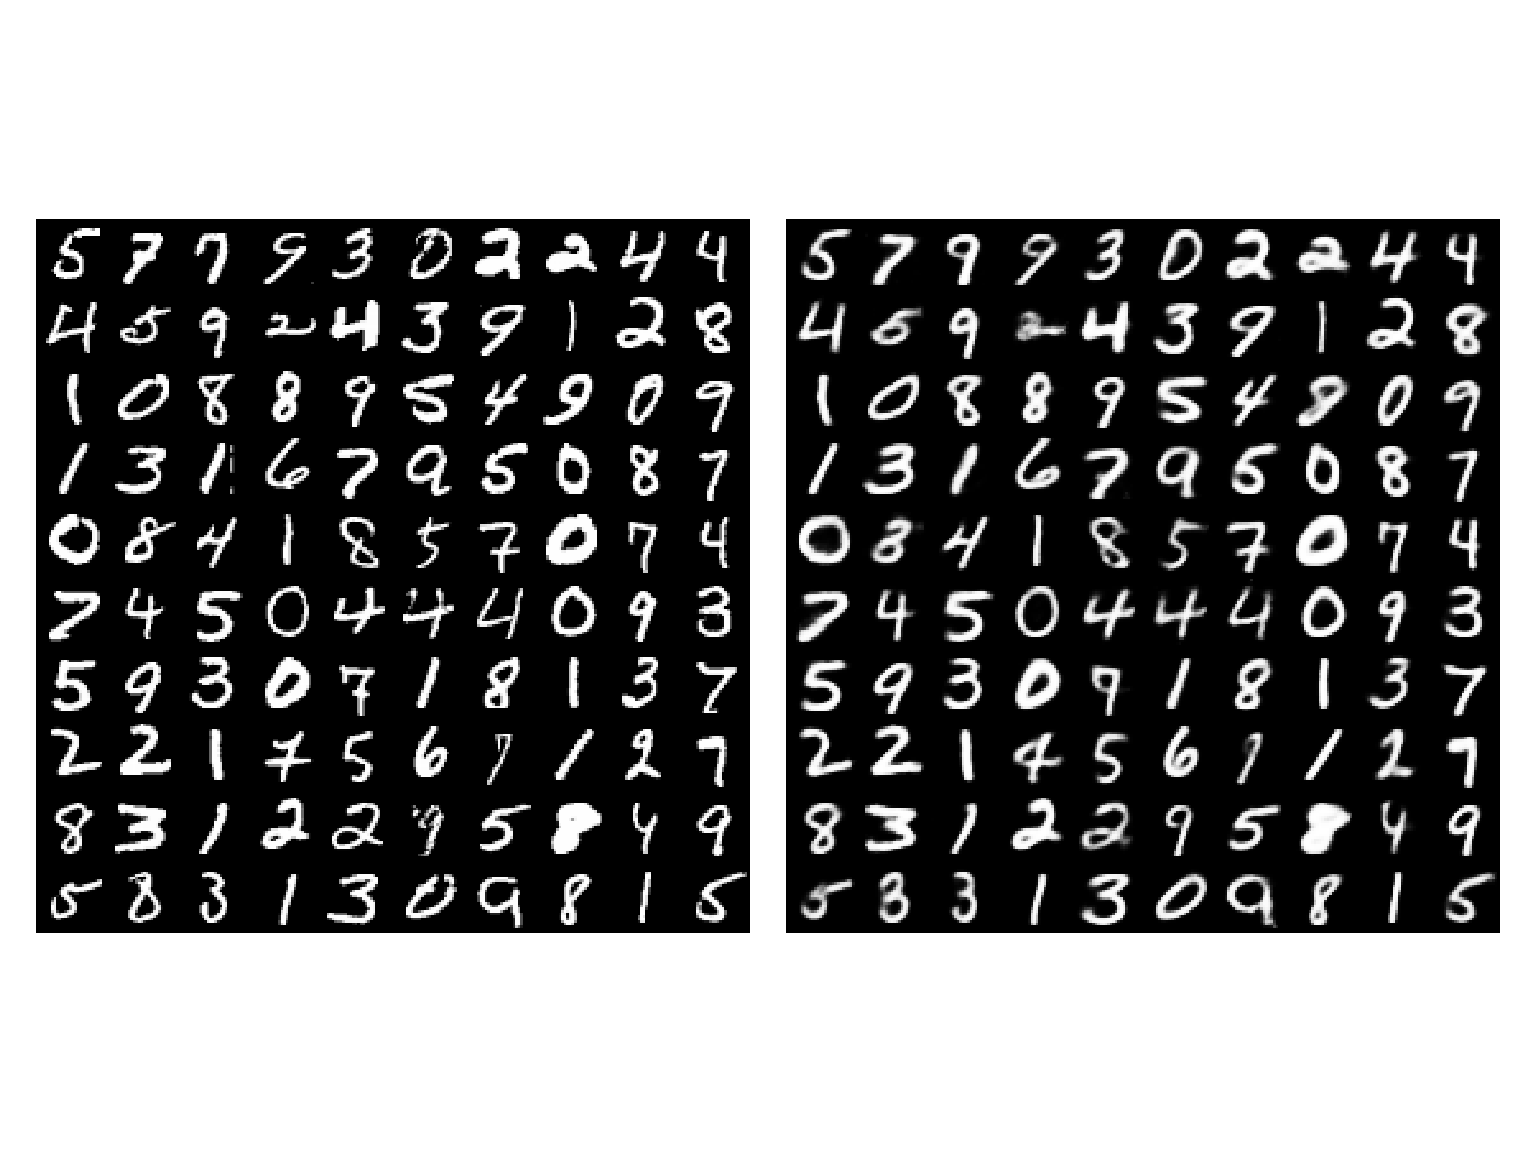
\includegraphics[height=200px]{includes/plots/dmvae/mnist/regenerated.png}
				\caption{Using DMVAE: Original(left) vs Reconstructed(right)}
				\label{fig:dmvae_mnist_regen}
			\end{figure}
			\begin{figure}[H]
				\centering
				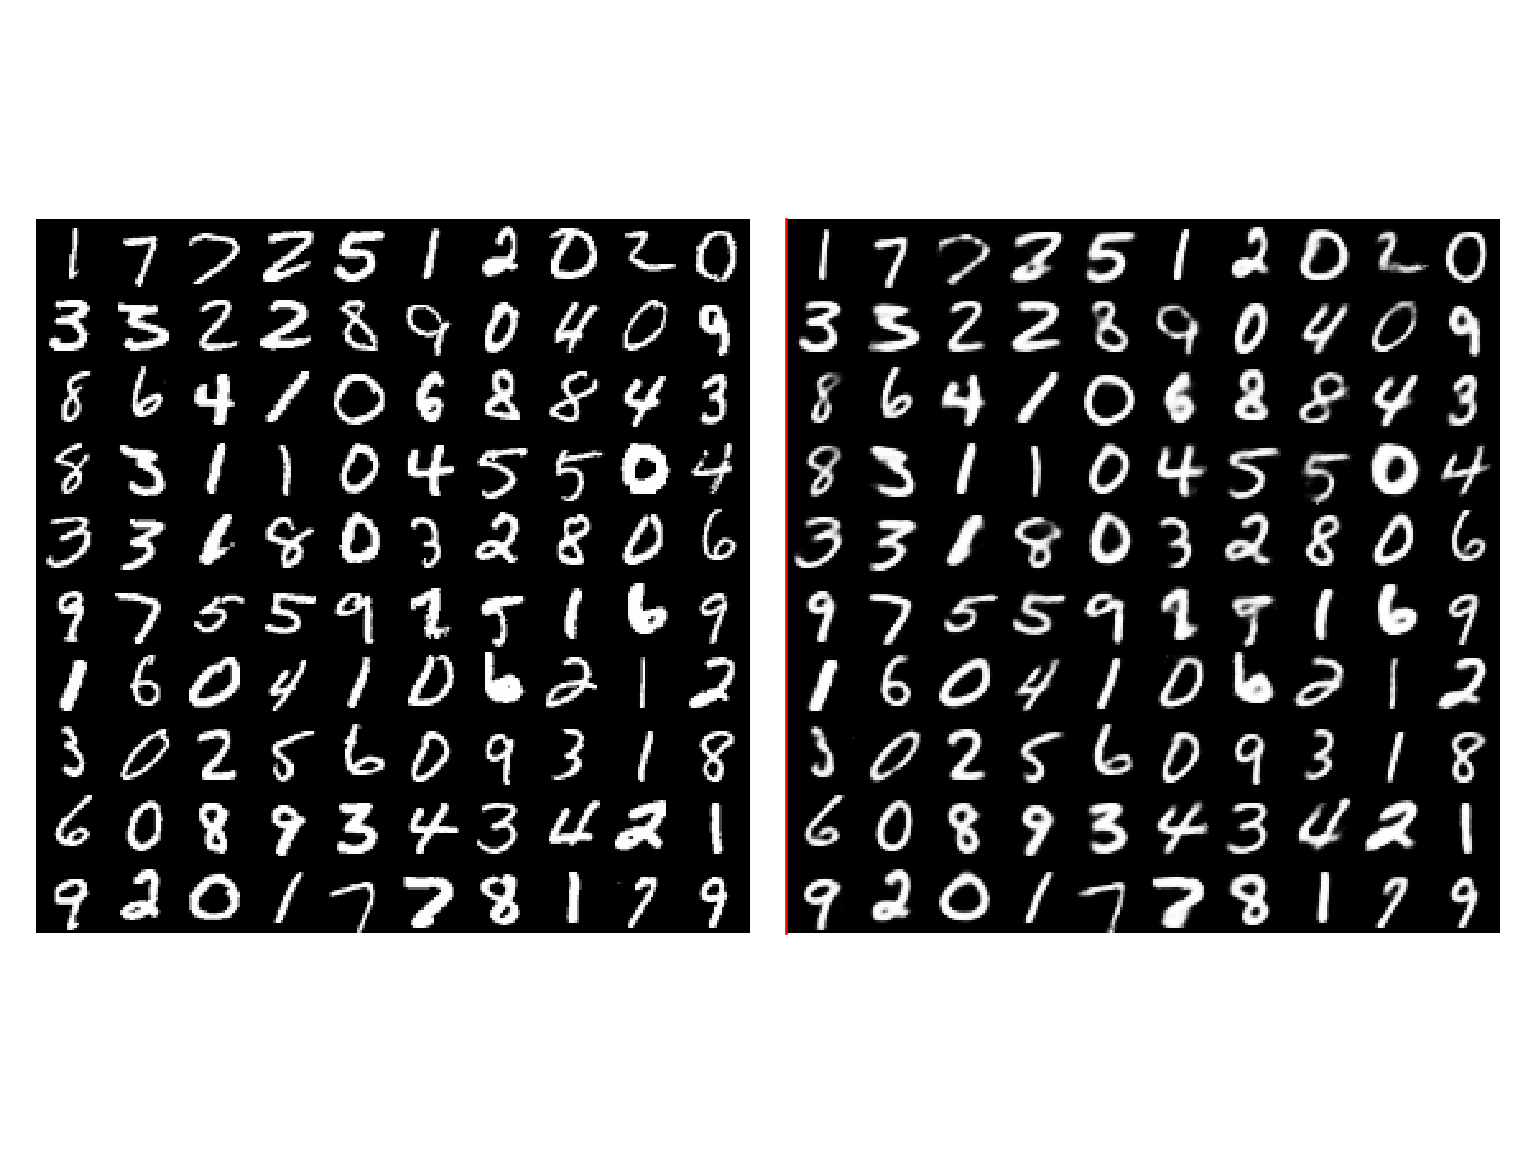
\includegraphics[height=200px]{includes/plots/vade/mnist/regenerated.png}
				\caption{Using VaDE: Original(left) vs Reconstructed(right)}
				\label{fig:vade_mnist_regen}
			\end{figure}

			Figures \ref{fig:dmvae_mnist_sampled} and \ref{fig:vade_mnist_sampled} show the comparison of performances in generating new images between DMVAE and VaDE. Each row corresponds to images generated as belonging to the same cluster by the model. It can be clearly seen that baring a few exceptions, the models produce extremely real looking images of digits, and hence can be used as powerful generative models.

			Moreover, in case of VaDE, we can see higher ambiguity between two clusters (both produce digit 1), which was not observed in our model.
			\begin{figure}[H]
				\centering
				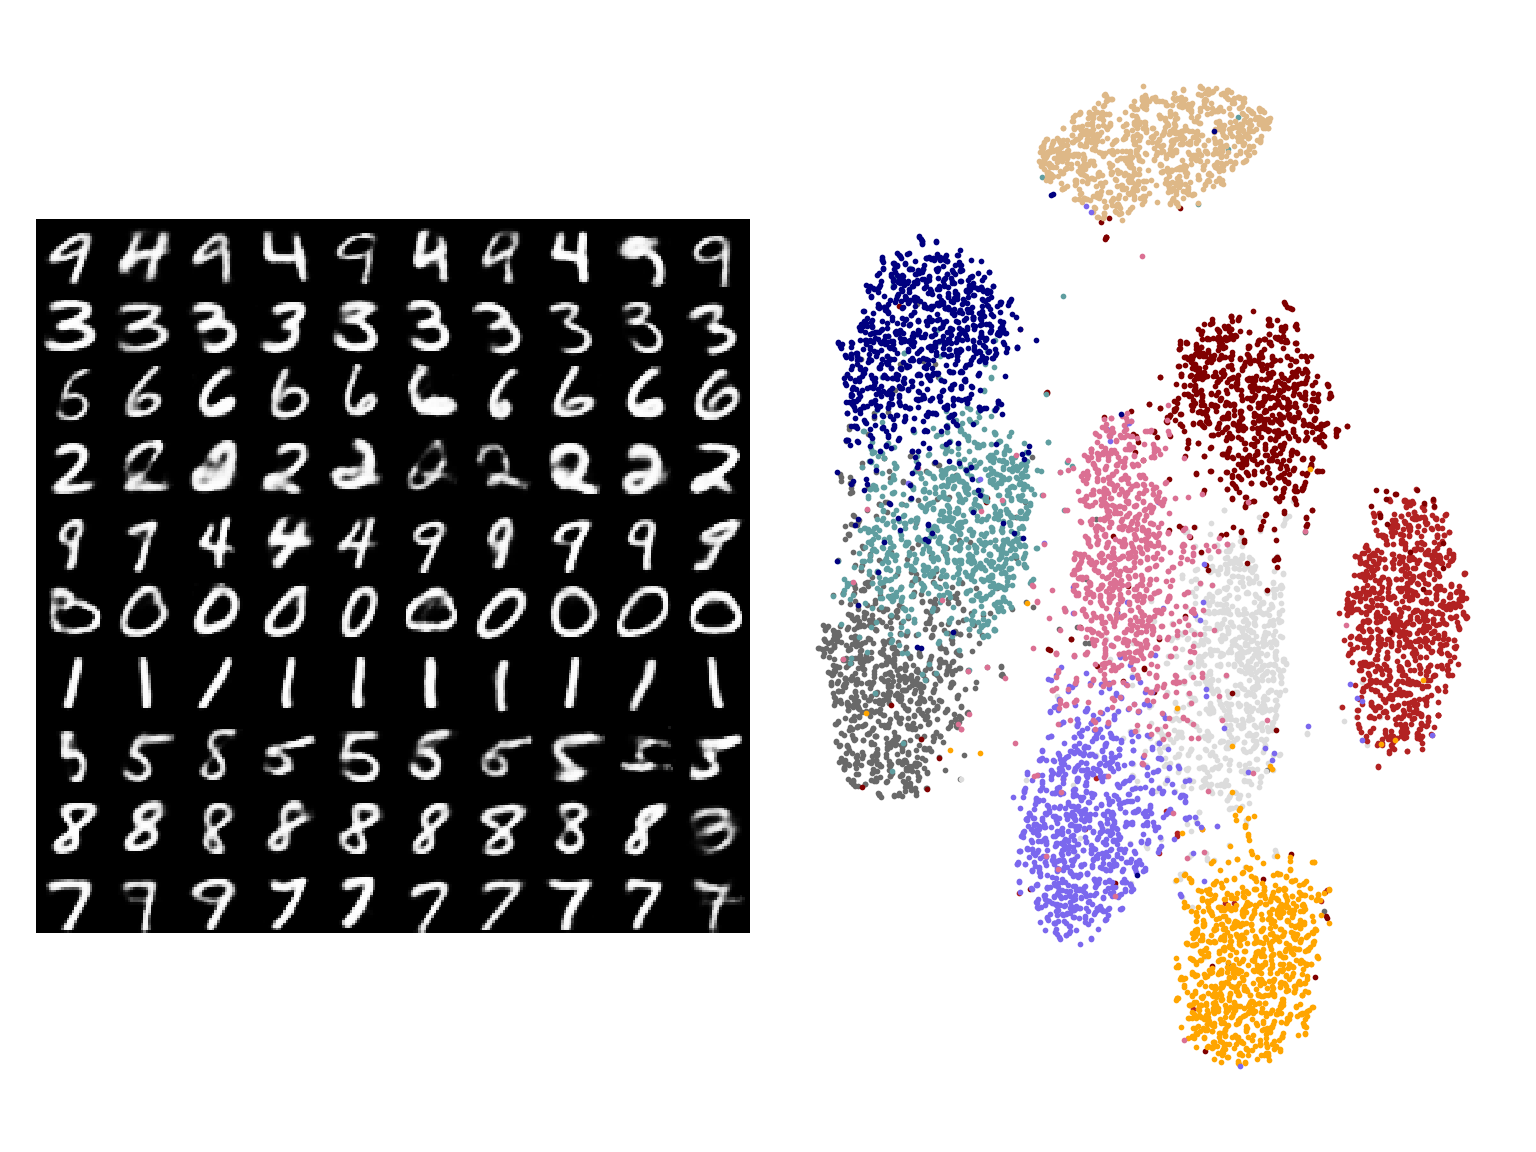
\includegraphics[height=200px]{includes/plots/dmvae/mnist/sampled.png}
				\caption{Using DMVAE: Generated Images(left) and tSNE plots(right)}
				\label{fig:dmvae_mnist_sampled}
			\end{figure}
			\begin{figure}[H]
				\centering
				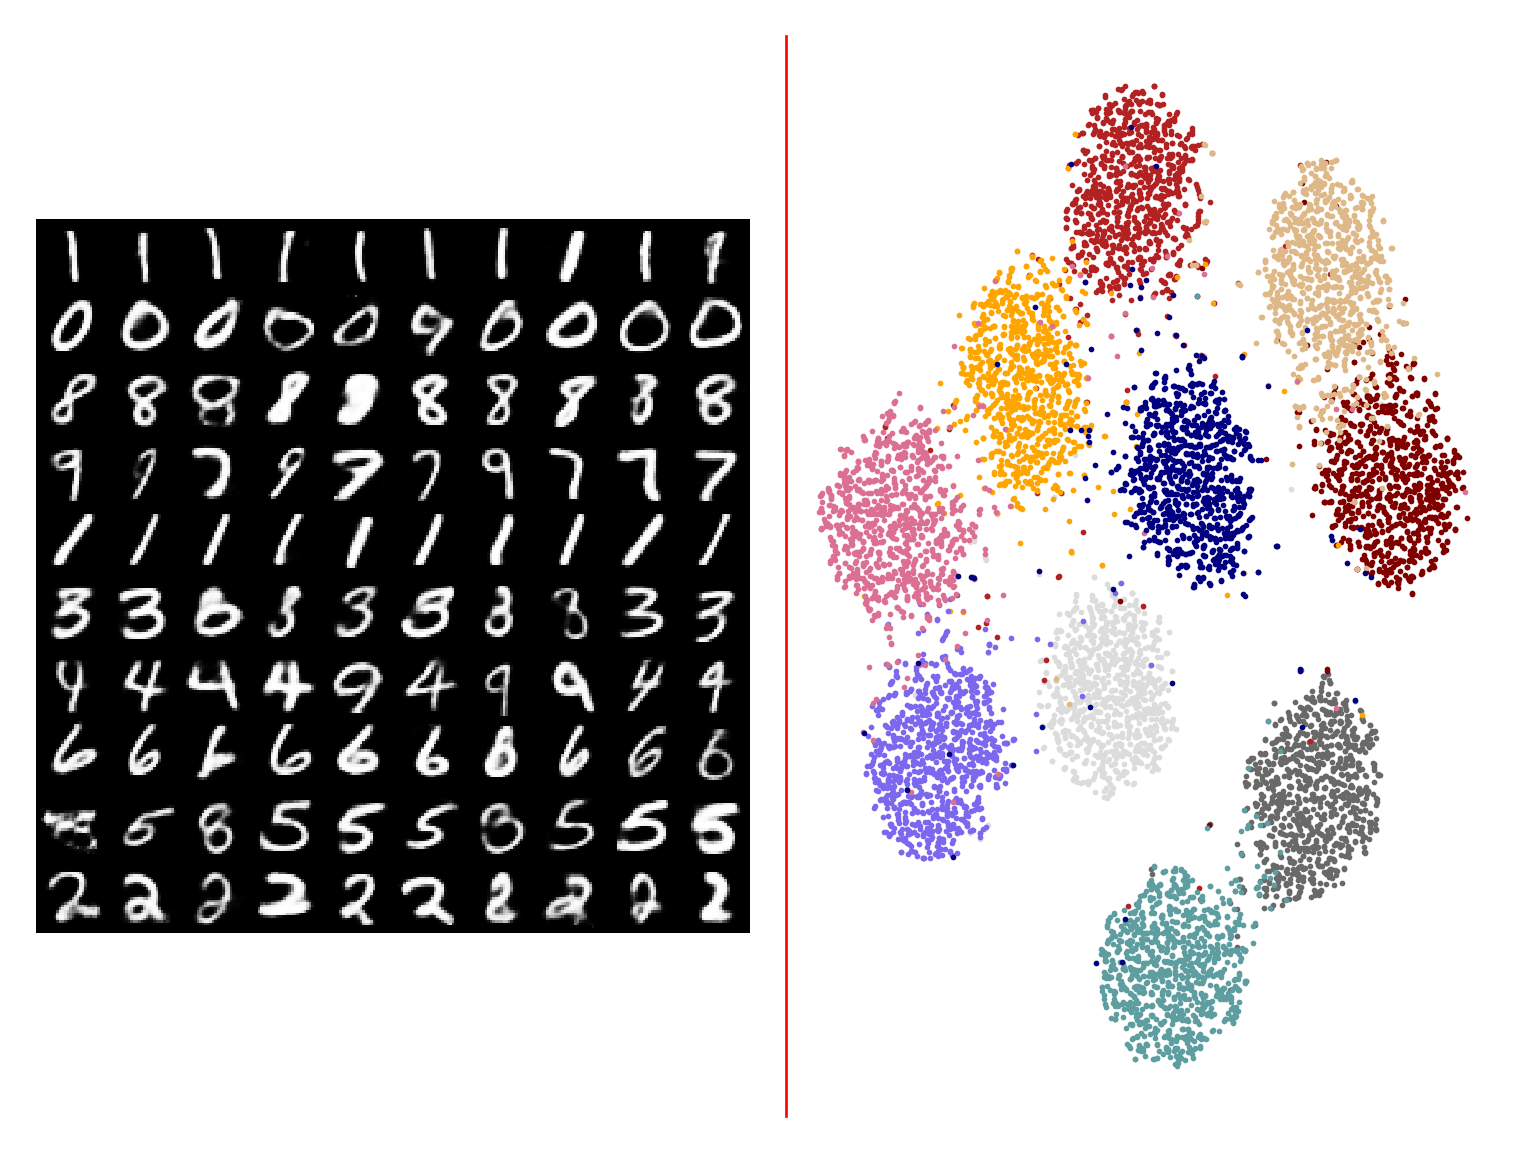
\includegraphics[height=200px]{includes/plots/vade/mnist/sampled.png}
				\caption{Using VaDE: Generated Images(left) and tSNE plots(right)}
				\label{fig:vade_mnist_sampled}
			\end{figure}

		\end{pssubsection}
		\begin{pssubsection}{Spiral Dataset}
			Spiral dataset is an artificial dataset used by us to test the performance of our models. The spiral dataset has complicated decision boundary shapes which are not easily learnt by most models. Our dataset consists of 5 classes and we again compare the reconstruction and generative powers of both DMVAE and VaDE models for this dataset.

			Figures \ref{fig:dmvae_spiral_regen} and \ref{fig:vade_spiral_regen} show the reconstructed datapoints by DMVAE and VaDE models respectively. Both models are able to reconstruct the points quite well, however, one interesting aspect to note is that the reconstructed points in DMVAE model suffer from very low variance and are tightly bound to their clusters, which is significantly higher in points reconstructed using VaDE model. Although this difference is quite minute, it verifies our claim that inference in DMVAE is better than that in VaDE.
			\begin{figure}[H]
				\centering
				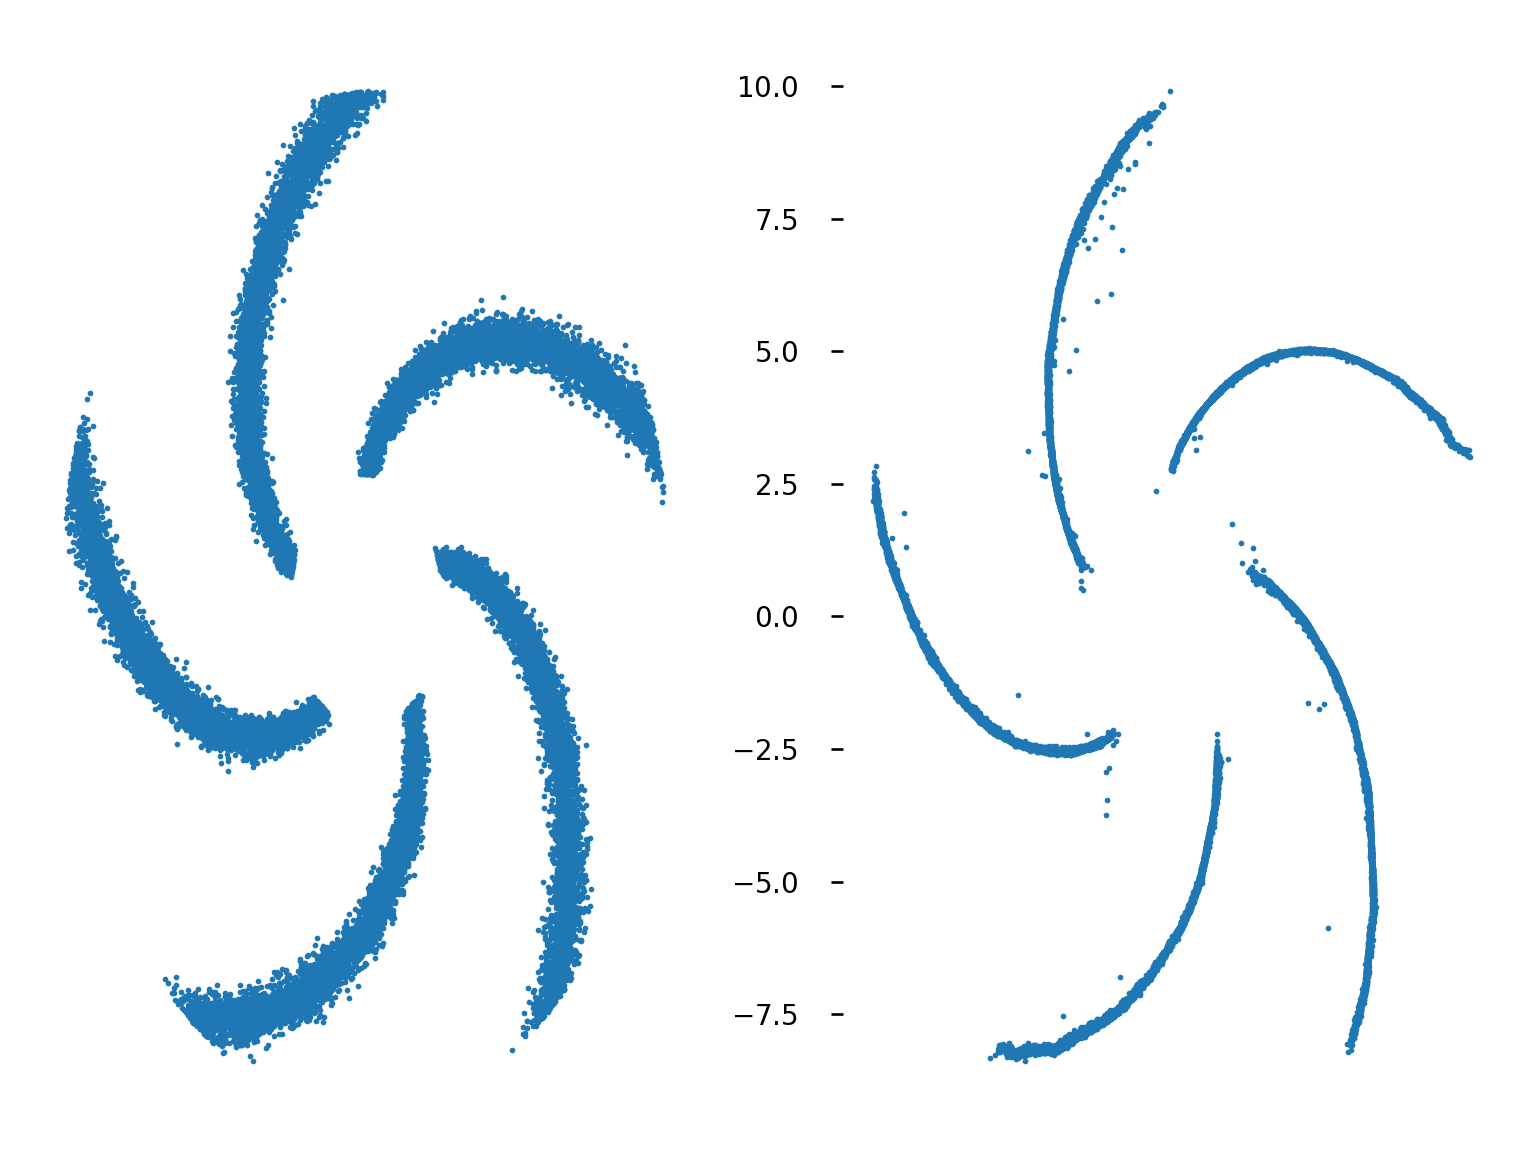
\includegraphics[height=200px]{includes/plots/dmvae/spiral/regenerated.png}
				\caption{Using DMVAE: Original(left) vs Reconstructed(right)}
				\label{fig:dmvae_spiral_regen}
			\end{figure}
			\begin{figure}[H]
				\centering
				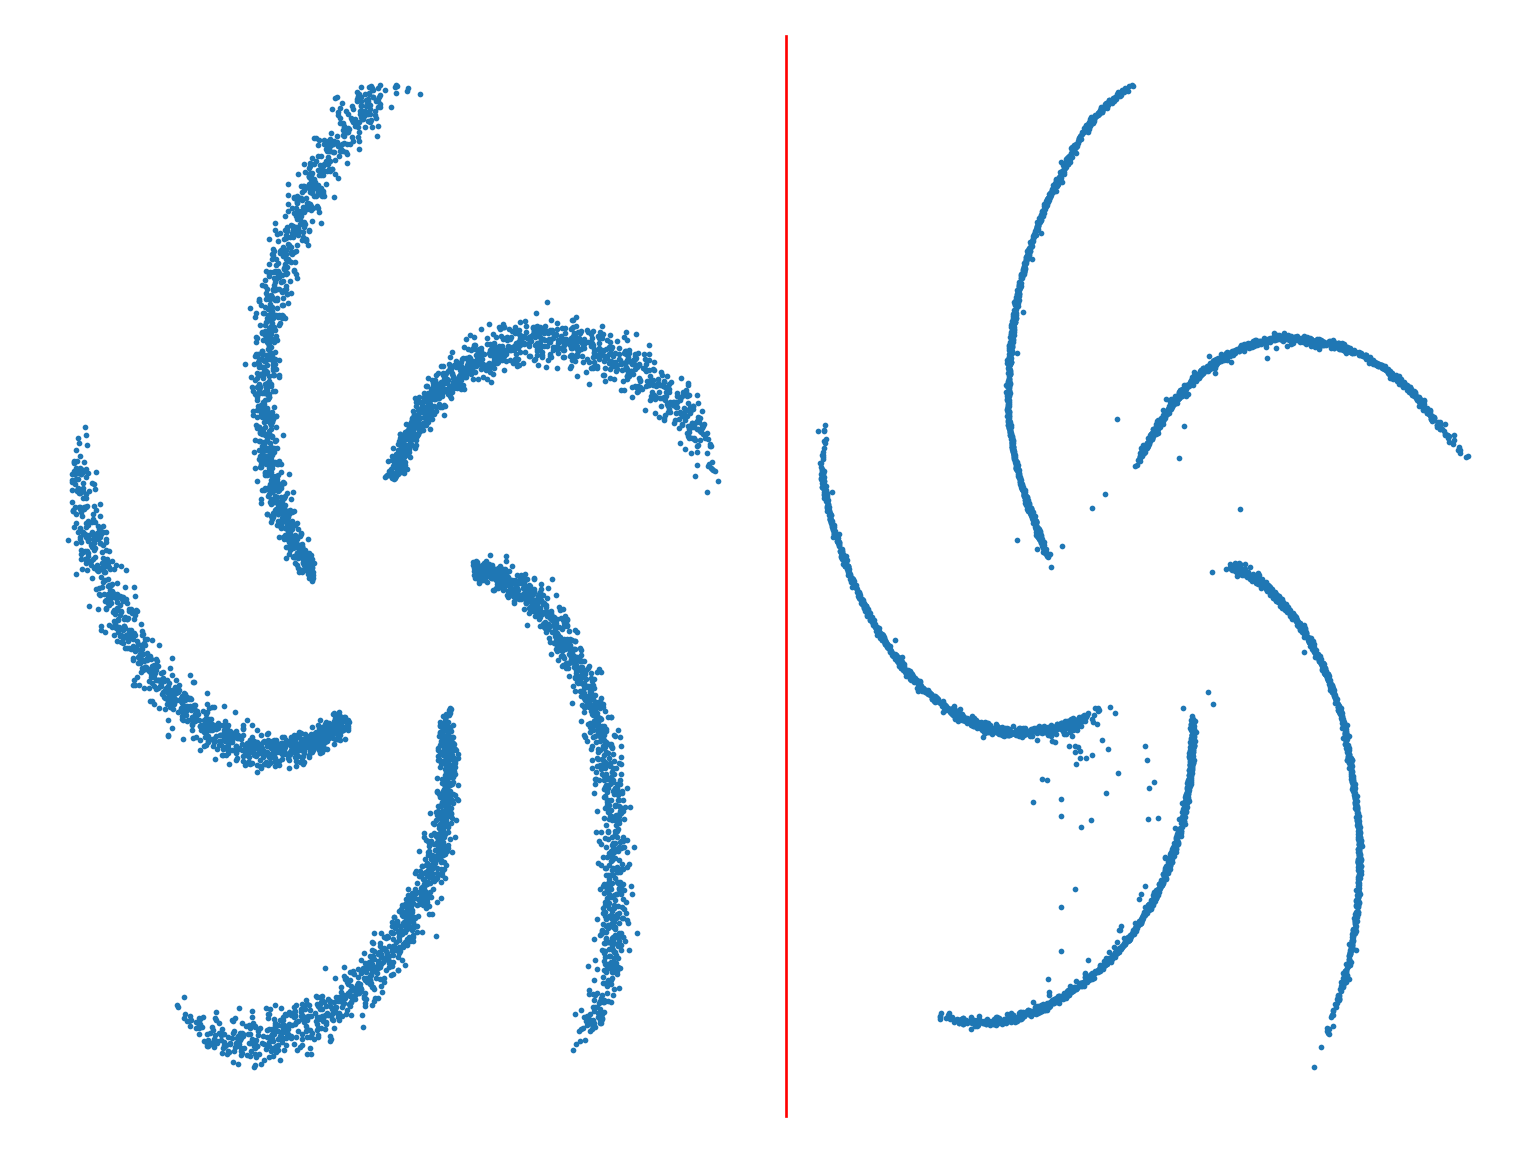
\includegraphics[height=200px]{includes/plots/vade/spiral/regenerated.png}
				\caption{Using VaDE: Original(left) vs Reconstructed(right)}
				\label{fig:vade_spiral_regen}
			\end{figure}

			Figures \ref{fig:dmvae_spiral_sampled} and \ref{fig:vade_spiral_sampled} show the points generated by DMVAE and VaDE models using spiral dataset. It is evident that the DMVAE model clearly outperforms VaDE model in this case, since VaDE is unable to distinguish between the green and blue clusters(see \ref{fig:vade_spiral_sampled}). On the other hand, DMVAE generates the points almost similar to real dataset and learns very well defined clusters. This proves that for general use cases, DMVAE is superior to VaDE.
			\begin{figure}[H]
				\centering
				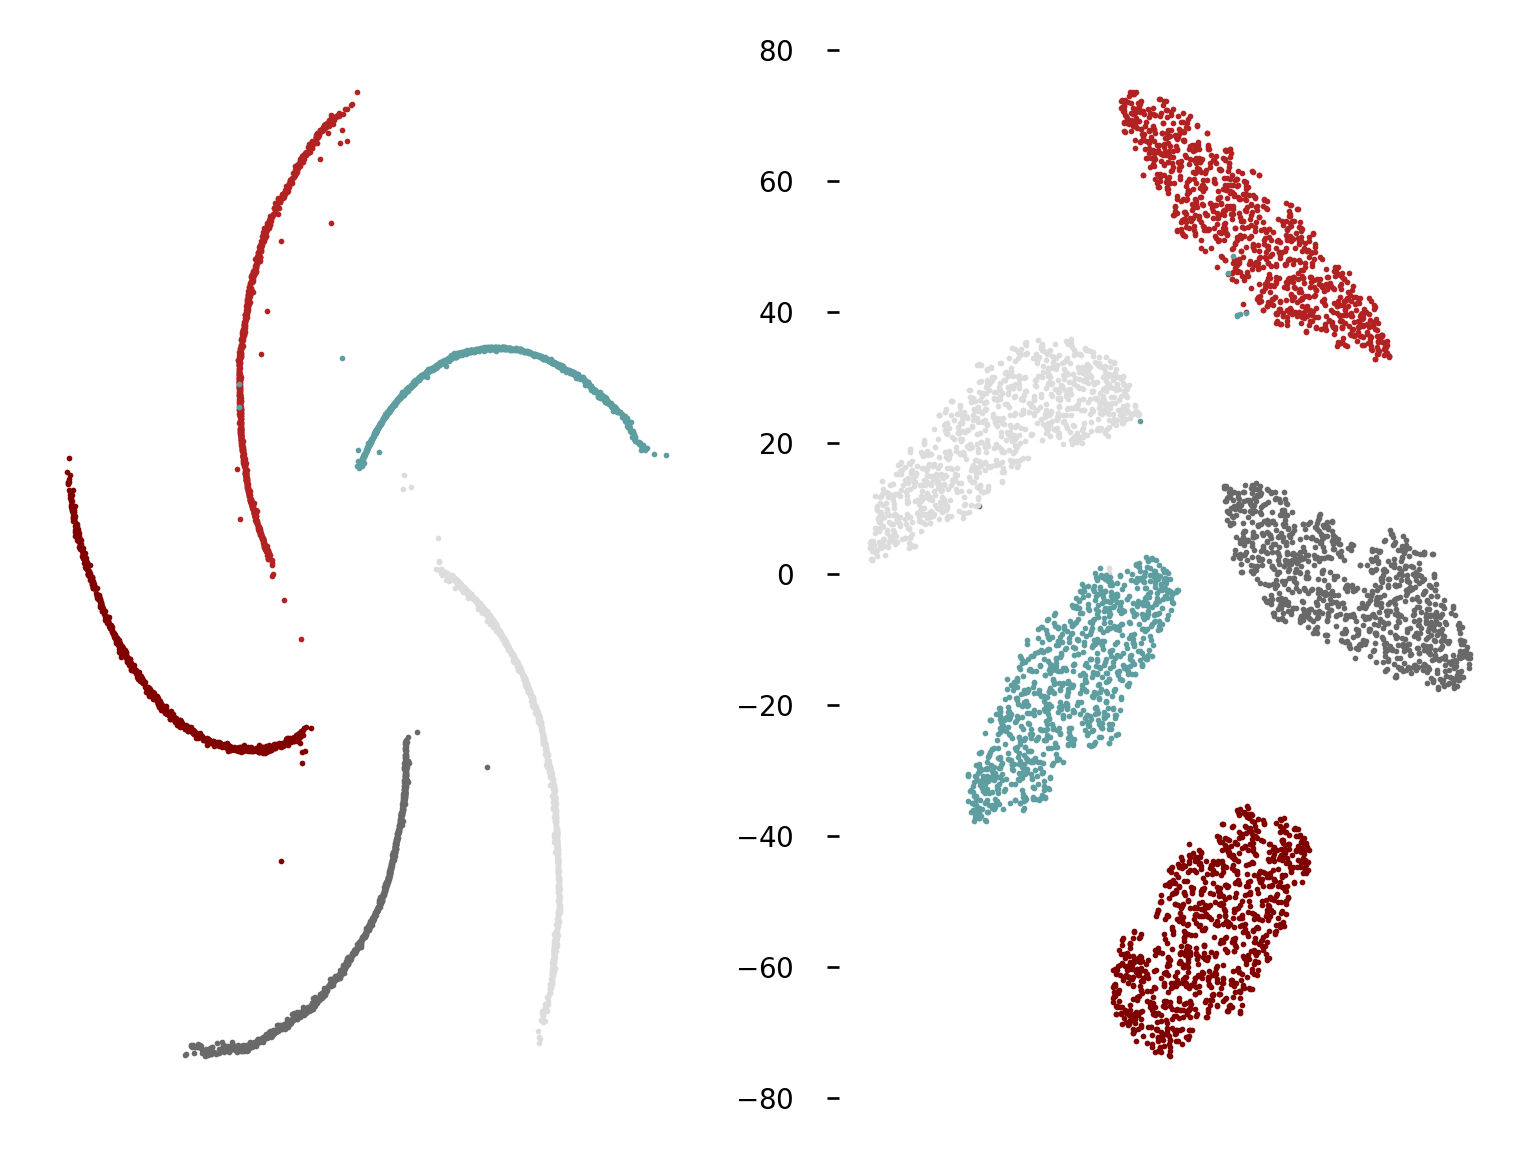
\includegraphics[height=200px]{includes/plots/dmvae/spiral/sampled.png}
				\caption{Using DMVAE: Generated Points(left) and tSNE plots(right)}
				\label{fig:dmvae_spiral_sampled}
			\end{figure}
			\begin{figure}[H]
				\centering
				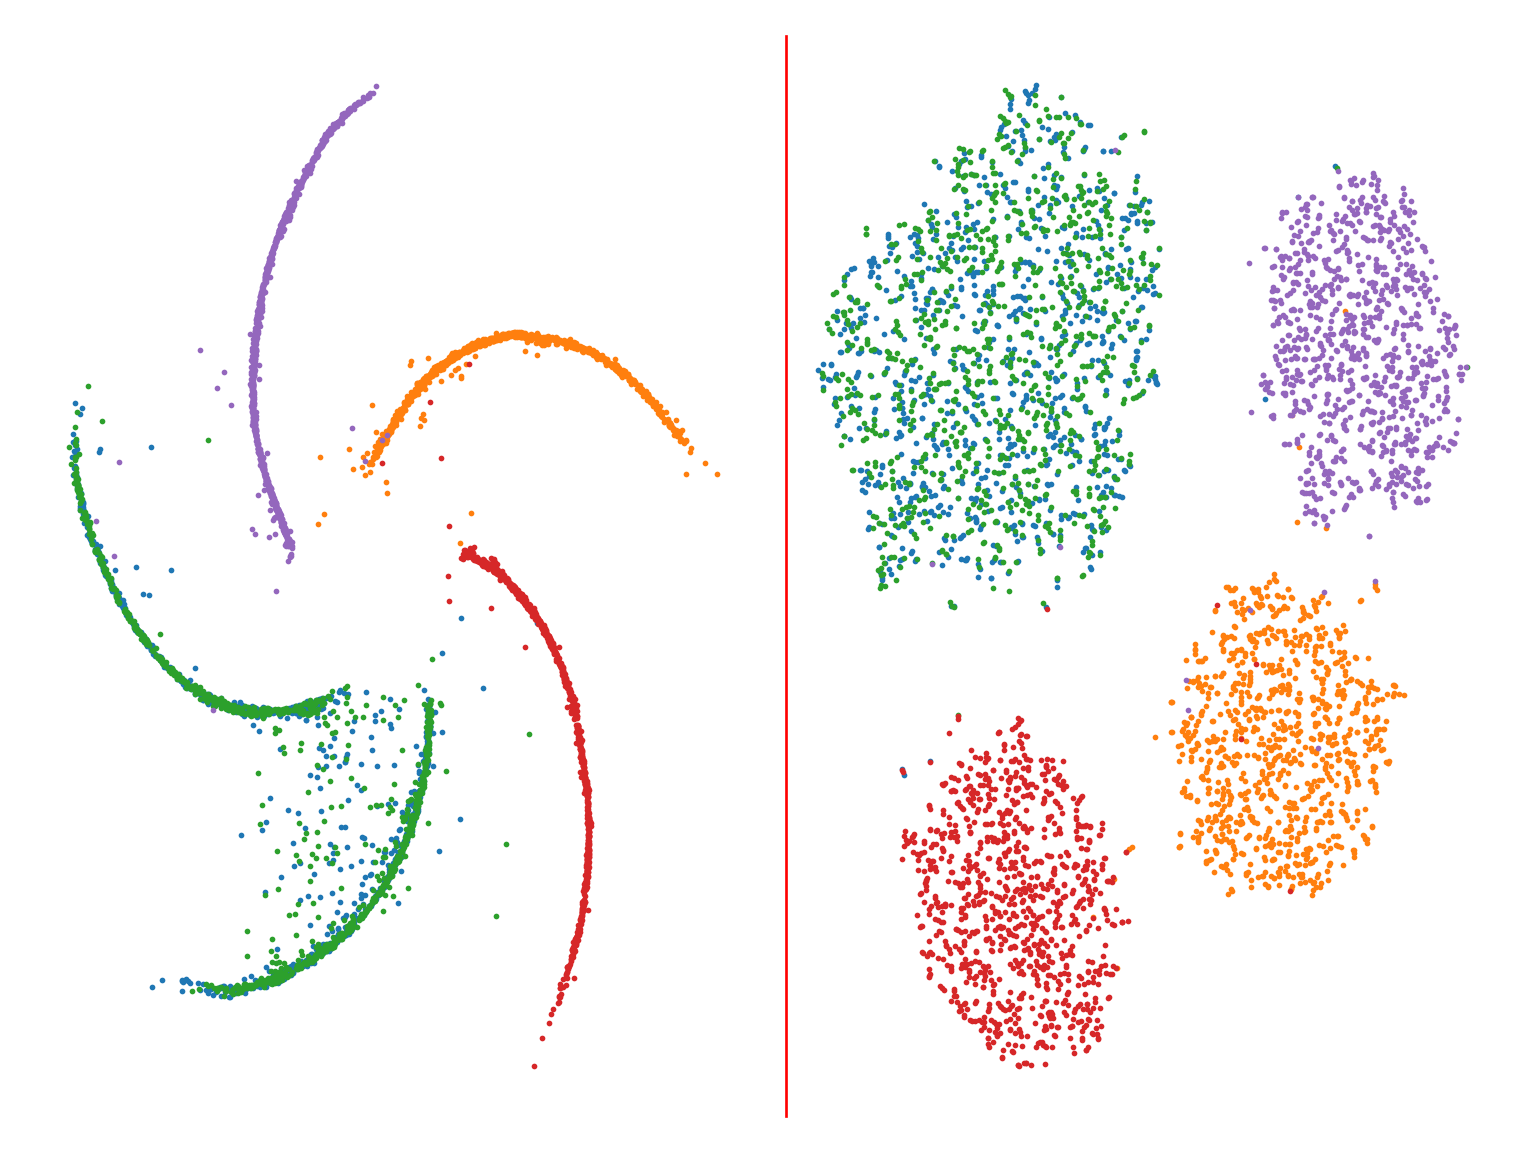
\includegraphics[height=200px]{includes/plots/vade/spiral/sampled.png}
				\caption{Using VaDE: Generated Points(left) and tSNE plots(right)}
				\label{fig:vade_spiral_sampled}
			\end{figure}
		\end{pssubsection}

		The biggest difference between VaDE and DMVAE is the training time and convergence rate. As a general trend, we found VaDE to converge in around 500-700 epochs, whereas DMVAE showed comparable results in only 200-300 epochs. In addition to this, the average training time for one epoch in case of VaDE was ~13s and in case of DMVAE was ~3.5s. We also observed, empirically, that VaDE performs poorly if there is no pretraining (details in the VaDE paper), but our model was more robust to initialization.

		For these reasons, we consider the DMVAE model to be better than VaDE for clustering in arbitrary shapes.
	\end{psubsection}

	\begin{psubsection}{Mixture of Experts Results}
		To measure the improvement provided by using Mixture of Experts with DMVAE as the gating function, we use a regression task. Each datapoint in MNIST dataset was annotated with a $K$-dimensional label, which was obtained by applying an affine transformation $f : \vX \rightarrow \vw\vX + \vb$ to the original $28\times28$ image. Here, $\vw$ and $\vb$ were chosen randomly, but were same for all points, thus ensuring that the final labels inherited the latent properties of input space. The same was done for Spiral dataset as well.

		First, we tried using a simple Gaussian Mixture Model as the gating function(\cite{NIPS1994_906}) using EM algorithm, where all the updates were manually calculated. However it proved to be extremely unstable and difficult to train since the probabilities quickly became 0 for higher dimensional spaces. Therefore, we had to discard using this algorithm. Nevertheless, we provide the code to implement the algorithm and are positive that the algorithm will perform well in lower dimensional spaces.

		\begin{table}
			\centering
			\begin{tabular}{c | l l | l l}
				& \multicolumn{2}{c|}{\bt{Spiral}}	& \multicolumn{2}{c}{\bt{MNIST}} \\ \hline
				\bt{Number of Dimensions}	& \bt{Deep MoE}	& \bt{DVMoE}		& \bt{Deep MoE}	& \bt{DVMoE} \\ \hline
				1							& 10.0424		& \bt{0.0312}		& \bt{28.4584}	& 34.0551 \\
				2							& 20.4247		& \bt{0.0434}		& \bt{209.028}	& \bt{208.142} \\
				5							& 180.117		& \bt{96.1049}		& 180.117		& \bt{96.1049}\\
			\end{tabular}
			\caption{Regression test results on Spiral and MNIST datasets; Deep MoE vs DVMoE}
			\label{tab:me-results}
		\end{table}

	\end{psubsection}

\end{psection}

\begin{psection}{Related Work}

\end{psection}

\begin{psection}{Conclusion}

\end{psection}

\bibliographystyle{plainnat}
\bibliography{main}

\end{document}

